%- in some cases search is still hard but the network operator might have an idea of what the path patterns might or might not look like - Done
%- example? - Done
%- a good way to express this is to add extra constraints of the form ... - Done
%- we formally define a subset of regexes that...?
%- algorithm
%- brief comparison with netgen
\section{Tactics} \label{sec:tactic}
Synthesizing a data plane translates to choosing paths from
the solution space of all paths for each reachability policy such
that the chosen paths satisfy all policies, e.g., waypoint traversal
and isolation. Datacenter topologies, e.g., fat-trees~\cite{fattree},
have numerous paths between edge switches to provide full bisection
bandwidth.  Thus, the solution space of paths for a pair of endpoints
is large.  For example, consider the fat-tree topology in
\Cref{fig:fattree}.  The number of paths under length 10 between two
edge switches in the same pod is 242 and between two edge switches in
different pods is 272.  If we consider the synthesis of $n$ packet
classes, the problem roughly translates to finding a solution in the
space of size $(242)^n$.
\begin{figure}
	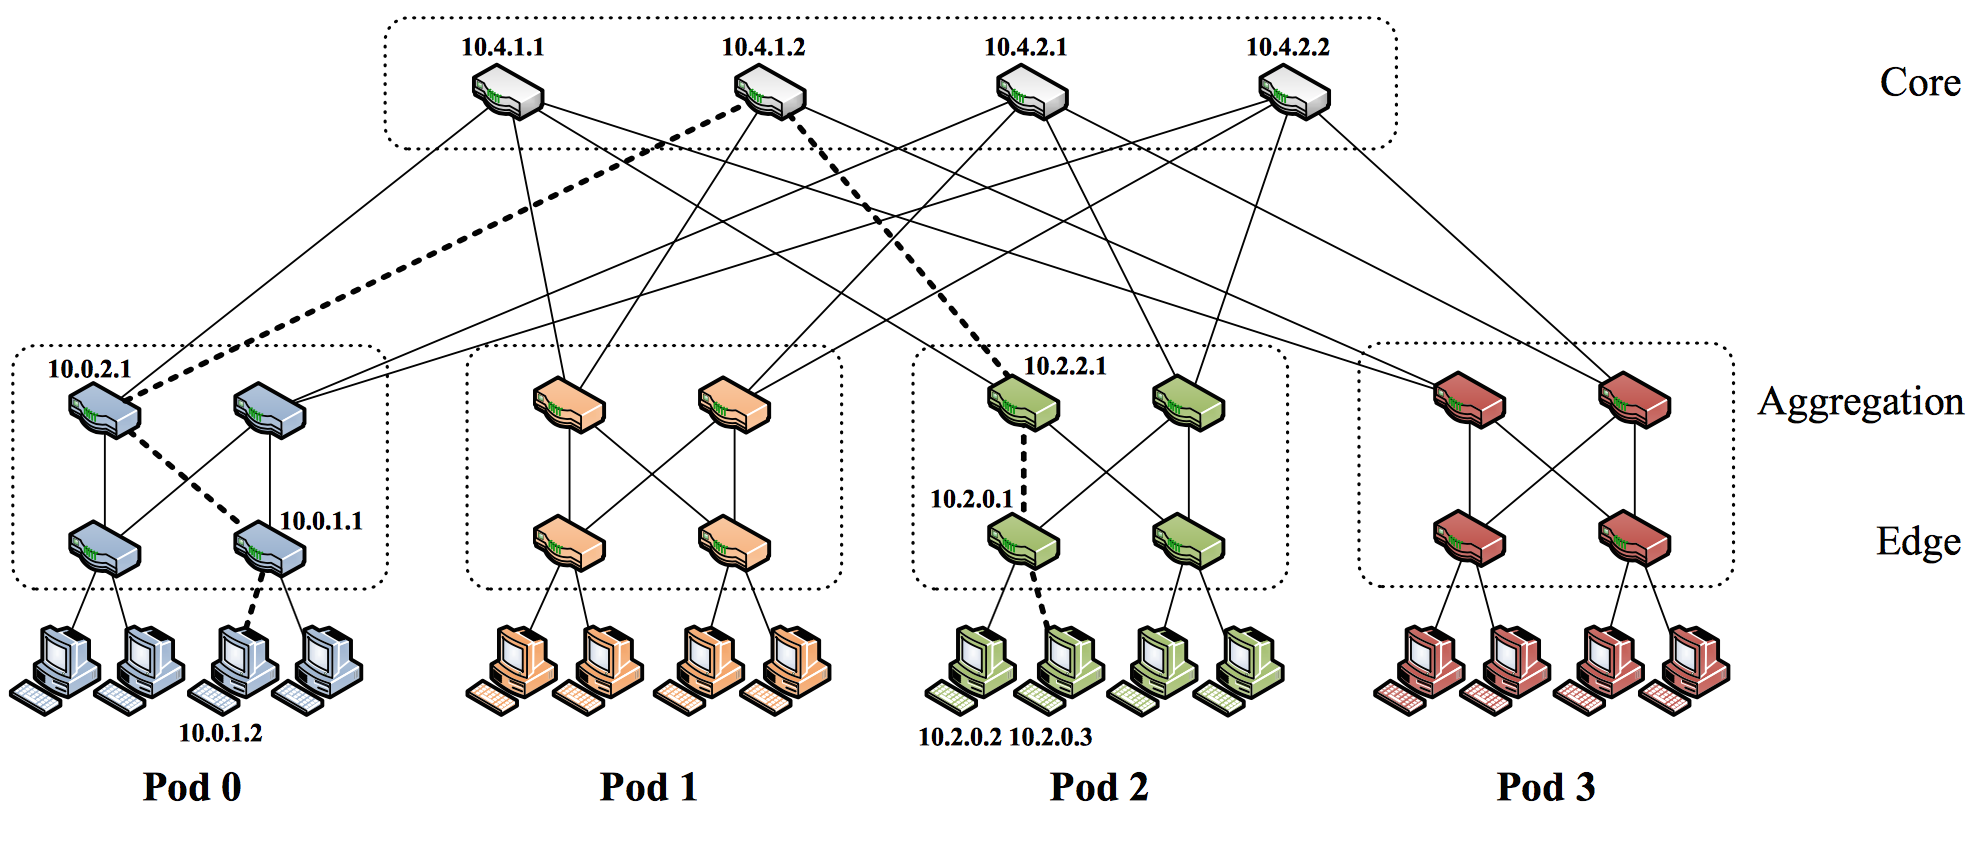
\includegraphics[width=0.9\columnwidth, right]{figures/fattree.png}
	\compactcaption{Fat Tree Topology with 3-level hierarchy.}
	\label{fig:fattree}
\end{figure}
Operators can leverage the network structure of topologies to reduce
the solution space by specifying undesirable path patterns.  For
example, the operator might require that a path between two edge switches in a
fat-tree does not traverse another edge switch.  This pattern doesn't
drastically reduce the set of possible paths due to the dense
interconnect between aggregate and core switches. 

We introduce \emph{tactics} (the name is inspired from the usage in SMT solvers, not 
proof assistants)
on labels; abstractions that allow a
network operator to impose restrictions on paths. 
We use the notion of mapping the set of switches to labels to 
have a coarse-grained way for specifying path patterns. Tactics on labels 
help create search strategies which can be used for groups
of packet classes instead of individual switch-level patterns which
lack generality.

 Let $Lb$ be the set of labels and $S$ be the set of switches in the topology. 
 Let $\phi : S \rightarrow Lb$ be the labeling function that maps each switch to a label in $Lb$. 
% One example for $\phi$ in the fat-tree topology in \Cref{fig:fattree} can be that we map all switches 
%therefore leveraging the hierarchical structure of the topology. 
For e.g., we can leverage the hierarchical structure of the fat-tree by
mapping all switches in the same level (core, aggregate or edge) to the same label.
A path $p$ is a word over the alphabet $S$. 
We define the path-labeling function $\Phi : S^* \rightarrow Lb^*$,  which maps each switch in the path to its corresponding 
 label. 
 For example, given the path $p = e1\ a2\ c3\ a4\ e2$, the path-labeling function function produces 
 $\Phi(p) = eacae$---maps each switch to its corresponding label.
 Here, $e$, $a$, and $c$ stand for edge, aggregate, and core respectively.

\subsection{Synthesis with Tactics}
%We use regular expressions and finite automaton to prune the constraints and impose restrictions on the path. The natural way for operators to specify tactics are using \emph{blacklists}, which specify what the path should not be. To express this in a intuitive manner, we use regular expressions on the set of labels to specify blacklists. For example, to blacklist paths from a edge switch to edge switch to not go through another edge switch, we can describe the tactic as $\neg (e .^* e .^* e)$ where the label of all edge switches is $e$. Another tactic is of the form $\neg (e (.)^4 a c .* e)$ which specifies we have a path of length 4, we do not go in the direction towards the core (as to reach the edge, the path would have to then go downwards from the core). 
Tactics are simple regular expressions over the set
 of labels and are used to blacklist certain path patterns.
Regular expressions have been previously used in tools like
NetGen~\cite{netgen} to specify the paths for a packet class.
While supporting full regular expressions is possible, it causes a blow-up in the solving time as further
constraints need to be added to the solver to ensure that a path satisfies the regular expression. 
Rather than specifying how the path must look like,
 we use regular expressions on switch labels to specify \emph{blacklists} i.e.,
what the path must \emph{not} look like. A tactic,
 for example, can blacklist paths from an edge switch to an edge switch that go through another edge switch. 
%\loris{we need a plot for the full regex thing to compare with Madhu, it would be great to repeat some of their experiments}

\subsubsection{Restricted Tactic Syntax} 
We specify tactics using a restricted set of regular expressions\footnote{
	It is a subset of star-free languages~\cite{starfree}.}
 that not only do not require extra constraints to be added,
but actually allow us to reduce the number of constraints in $\Psi$.
Tactics are regular expressions described by the following grammar:
$$\begin{array}{rcl}
R  &  :=  &  \neg (l_{src} .^i C .^* l_{dst}) \\
C  &  :=  &  \varepsilon \mid l_1 \mid l_1 l_2\\
\end{array}$$
where $l_i\in Lb$ and $l_{src}, l_{dst}$ are used to specify the labels of the source switch 
and destination switch, respectively.
Since our goal is to blacklist paths, we allow regular expressions to be negated at the outer level. 
\begin{example}
 $\neg (e .^i c .^* e)$ indicates that the path must not contain a core switch at the $(i+1)^{th}$ step. 
 Similarly, $\neg (e .^i .^* e)$ indicates that the path connecting two edge switches should have a length $ < i + 1$. 
\end{example}

Let $\pi = sw_0\ldots sw_k$ be a path for packet class $pc$
and let its labeling be $\Phi(\pi)= a_0\ldots a_k$.
We say that $\pi$ satisfies a tactic $R$,  $\Phi(\pi) \in L(R)$, if the following
holds:
\begin{compact2itemize}
\item $\Phi(\pi) \in L(\neg R)$ iff $\Phi(\pi) \not\in L(R)$;
\item $\Phi(\pi) \in L( l_{src} .^i .^* l_{dst})$ iff $k\geq i+1$, $l_{src}= a_0$, and $l_{dst}= a_k$; 
\item $\Phi(\pi)  \in L (l_{src} .^i l.^* l_{dst})$ iff $k\geq i+2$, $l_{src}= a_0$, $l_{dst}= a_k$, and $a_{i+1}=l$;
\item $\Phi(\pi)  \in L( l_{src} .^i l_1 l_2.^* l_{dst})$ iff $k\geq i+3$, $l_{src}= a_0$, $l_{dst}= a_k$, $a_{i+1}=l_1$, and $a_{i+2}=l_2$.
\end{compact2itemize}
In \Name, operators can specify conjunctions of tactics which adhere to the restricted 
syntax and the synthesis algorithm is modified to enforce the tactics. 
\begin{example}
The ``No Edge'' tactic ensures that a edge-edge path
cannot traverse another edge switch. It is expressed using conjunctions of tactics:
$\neg (e .^* e .^* e)\equiv \bigwedge \limits_{i=0}^{i=\mu-2} \neg (e .^i e .^* e)$ where $\mu$ is the limit on path length. 
The ``Valley-free'' Tactic:  $\neg (e .^5 .^* e)$ $\wedge \neg (e .^* e .^* e)$  
ensures that a edge-edge path is of the form $e-a-c-a-e$. 
\end{example}
Paths used in production datacenter networks adhere to both these
tactics~\cite{vl2-sigcomm09,jupiterrising-sigcomm15}. Such paths are
simple and make networks easy to manage and
troubleshoot~\cite{benson:complexity:nsdi2009}.

\subsubsection{Modified Synthesis Algorithm with Tactics}
In our synthesis algorithm, the reachability-propagation constraints (\Cref{eq:bckprop}) 
construct the path from destination to source. We use tactics to prune these constraints, so that
the path synthesized satisfies the tactic regular expression.  

The tactic set $\Gamma = \{(R_1, pc_1), \ldots, (R_n, pc_n)\}$
specifies that tactic $R_i$ is applied on packet class $pc_i$ where 
$pc_1, \ldots, pc_n$ $\in PC$ and $R_1,\ldots,R_n$ are regular
expressions satisfying the restricted tactic syntax. 
Given a tactic $R$ applied to a packet class $pc$, 
we define $\Psi_T(R,pc)$ as the additional SMT constraints used for 
synthesis such that  $(\Psi \wedge\ \bigwedge\limits_{(R, pc) \in \Gamma} \Psi_T(R,pc))$ 
is provided as input to the SMT solver.
	Note that $\Psi_T(R,pc)$ is presented as additional SMT 
constraints only for clarity. 
In practice, the modified synthesis algorithm will remove constraints for each 
$(R,pc)\in \Gamma$.
%In the first
%two cases, we remove some of the reachability constraints by adding negated unit clauses, 
%while we modify these constraints for the next two cases.
%To incorporate tactics in the path for packet class $pc$, we need to modify these constraints. For a path $\pi = sw_0 \ldots sw_k$ and labeling $\Phi(\pi) = a_0 \ldots a_k$, we describe the modifications of the constraints for each type of tactic.
%\loris{this part needs revision. Every time you say we remove constraints, but it actually looks like you are adding extra constraints
%of the form not(..)}

\noindent\textbf{Type 1.} For a tactic $R$ of the form $\neg (l_{src} .^i .^* l_{dst})$ applied to $pc$: 
\begin{equation} \label{eq:type1}
	\Psi_T(R, pc) = ~ \forall sw,k \geq i + 1. (sw,pc,k) \notin Reach
\end{equation}
This tactic restricts the path to a length $ < i + 1$. Thus, we can remove the reachability constraints  of \Cref{eq:bckprop} 
for all the tuples $(sw,pc,k) \notin Reach$ satisfying \Cref{eq:type1}
as they cannot contribute to any path satisfying the tactic.  

\noindent\textbf{Type 2.} For a tactic $R$  
of the form $\neg (l_{src}  .^i l .^* l_{dst})$ applied to $pc$:
\begin{multline} \label{eq:t1}
\Psi_T(R,pc) = \forall sw.~ \phi(sw) = l ~\wedge~ sw \not= dst \implies \\ 
(sw, pc, i + 1) \notin Reach
\end{multline}
The tactic ensures that a switch with label $l$ cannot be reached in $i+1$
steps, except if $l = l_{dst}$. In that case,
only the destination switch with label $l$ can be reached in $i+1$ steps as 
the path with labeling $l_{src}.^i l_{dst}$ satisfies the tactic. If $l \not= l_{dst}$, then
all switches with label $l$ cannot be reached in $i+1$ steps. For all tuples
$(sw, pc, i+1) \notin Reach$ satisfying \Cref{eq:t1}, we can remove the reachability constraints of \Cref{eq:bckprop}.


\noindent\textbf{Type 3.} For a tactic $R$  
of the form $\neg (l_{src}  .^i l_1 l_2 .^* l_{dst})$ applied to $pc$: 
\begin{multline} \label{eq:t3}
\Psi_T(R,pc) = \forall n_1, n_2.~\phi(n_1) = l_1~\wedge~ \phi(n_2) = l_2 ~\wedge~ n_2 \not=dst \\  \implies 
\neg (Reach(n_1, pc, i + 1) \wedge Fwd(n_1, n_2, pc))
\end{multline}
This tactic ensures that a switch with label $l_1$ at $i+1$ in the path
will not forward the packet to a switch with label $l_2$ (unless $n_2$ is the destination). 
To enforce this, we modify the \Cref{eq:bckprop} and remove all $l_1\rightarrow l_2$
edges at position $i+1$ in the path for which the switch with label $l_2$  is not the destination.  

%-> if a path is solution of modified constraint it satisfies regex
%<- if a path is solution of original constraints and satisfies regex, then it's a possible solution of modified constraints.

%Thm 6.1: Given a tactic R for the class pc, if \Pi |= \psi /\ Psi_R, then for every (\pi,pc)\in \Pi, \pi|=R (written a  bit better)
%
%Thm 6.2: Given a tactic R for the class pc, 
%if \Pi |= \psi, 
%and for every (\pi,pc)\in \Pi, \pi|=\psi_R,
%\Pi |= Psi_R.
We now state the soundness and completeness  
of the synthesis algorithm with tactics. 
Let $(Fwd, Reach)$ be a model of $\Psi$ and 
$\Pi = \texttt{paths}$ $(Fwd,$ $Reach)$ be the set
of induced paths (from Definition \ref{def:Pi}).
\begin{theorem}[Soundness]
	For a tactic set $\Gamma$, if $(Fwd, Reach) \models \Psi \wedge \bigwedge\limits_{(R, pc) \in \Gamma} \Psi_T(R,pc)) $, 
	then $\forall (R, pc) \in \Gamma. ~\forall(\pi', pc') \in \Pi. ~pc = pc' \implies \Phi(\pi') \in L(R)$.
\end{theorem}
\iffull
\begin{proof}
	\textbf{Assume} $\exists (R,pc) \in \Gamma$ such that $(\pi, pc) \in \Pi$ and $\Phi(\pi) \not\in L(R)$.
	Consider the three types of tactics for $R$: \newline
	\textbf{Type 1}: $R = \neg (l_{src} .^i .^* l_{dst})$ \\
	$\Phi(\pi) \not\in L(R)$ $\implies$ $\Phi(\pi) \in L(l_{src} .^i .^* l_{dst})$. \\
	Thus, $\pi = src\ sw_1 \ldots sw_i \ldots dst$. \\
	Therefore,  $(dst, pc, k_{dst}) \in Reach, k_{dst} \geq i + 1$. \\
	However, $(Fwd, Reach) \models \Psi_T(R, pc) \implies (Fwd, Reach) \models \forall sw,k \geq i + 1. (sw,pc,k) \notin Reach$.\\
	Contradiction, as $\exists sw, k \geq i + 1. (sw,pc,k) \in Reach$.
	\newline
	\newline
	\textbf{Type 2}: $R = \neg (l_{src} .^i \ l \ .^* l_{dst})$ \newline
	$\Phi(\pi) \not\in L(R)$ $\implies$ $\Phi(\pi) \in L (l_{src} .^i \ l \ .^* l_{dst})$. \\
	Thus, $\pi = src\ sw_1 \ldots sw_i \ sw_{i+1} \ldots dst$ such that $\phi(sw_{i+1}) = l$. Also $sw_{i+1} \not=dst$ (dst has to be the last switch in $\pi$)\\
	Therefore,  $(sw_{i+1}, pc, i+1) \in Reach$. \\
	However,
	$(Fwd, Reach) \models \Psi_T(R, pc) \implies (Fwd, Reach) \models \forall sw.~ \phi(sw) = l ~\wedge~ sw \not= dst \implies  (sw, pc, i + 1) \notin Reach$. \\
	Contradiction, as $\exists sw. ~ \phi(sw) = l ~\wedge~ sw \not= dst \wedge (sw,pc,i+1) \in Reach$.
	\newline \newline
	\textbf{Type 3}: $R = \neg (l_{src} .^i \ l_1 \ l_2 \ .^* l_{dst})$ \newline
	$\Phi(\pi) \not\in L(R)$ $\implies$ $\Phi(\pi) \in L (l_{src} .^i \ l_1 \ l_2 \ .^* l_{dst})$. \\
	Thus, $\pi = src\ sw_1 \ldots sw_i \ sw_{i+1} \ sw_{i+2} \ldots dst$ such that \newline $\phi(sw_{i+1}) = l_1, \phi(sw_{i+2}) = l_2$. Also $sw_{i+2} \not=dst$ (dst has to be the last switch in $\pi$)\\
	Therefore,  $(sw_{i+1}, pc, i+1) \in Reach \wedge (sw_{i+1}, sw_{i+2}, pc) \in Fwd$. \\
	However,
	$(Fwd, Reach) \models \Psi_T(R, pc) \implies (Fwd, Reach) \models \forall n_1, n_2.~\phi(n_1) = l_1~\wedge~ \phi(n_2) = l_2 ~\wedge~ n_2 \not=dst  \implies 
	\neg (Reach(n_1, pc, i + 1) \wedge Fwd(n_1, n_2, pc))$. \\
	Contradiction, as $\exists n_1. n_2. ~\phi(n_1) = l_1~\wedge~ \phi(n_2) = l_2 ~\wedge~ n_2 \not=dst \wedge Reach(n_1, pc, i + 1) \wedge Fwd(n_1, n_2, pc)$. 
\end{proof}
\fi

\begin{theorem}[Completeness]
For a tactic set $\Gamma$, if $~\Pi \models \Psi$ and 
$\forall (R, pc) \in \Gamma. ~\forall(\pi', pc') \in \Pi. ~pc = pc' \implies \Phi(\pi') \in L(R)$
then $\forall (R, pc) \in \Gamma. (Fwd, Reach) \models \Psi_T(R, pc)$.
\end{theorem}
\iffull
\begin{proof}
	\textbf{Assume} $\exists (R, pc) \in \Gamma$ such that $(\pi, pc) \in \Pi$ and \newline 
	$(Fwd, Reach) \not\models \Psi_T(R,pc)$.
	Consider the three types of tactics for $R$: \newline
	\textbf{Type 1}: $R = \neg (l_{src} .^i .^* l_{dst})$ \newline
	$(Fwd, Reach) \not\models \Psi_T(R, pc) \implies (Fwd, Reach) \not\models \forall sw,k \geq i + 1. (sw,pc,k) \notin Reach$ \newline
	Therefore $\exists sw, k \geq i + 1. (sw,pc,k) \in Reach$. \\
	Therefore, $\Phi(\pi) \in L(l_{src}\ .^i \ .^* \ \phi(sw) \ .^* \ l_{dst}) \implies \Phi(\pi) \in L(l_{src} .^i .^* l_{dst}).$\\
	Contradiction, as $\Phi(\pi) \in L(R)$.
	\newline 
	\newline 
	\textbf{Type 2}: $R = \neg (l_{src} .^i \ l \ .^* l_{dst})$ \newline
	$(Fwd, Reach) \not\models \Psi_T(R, pc)$ $\implies$ $(Fwd, Reach) \not\models$ \newline $\forall sw.~ \phi(sw) = l ~\wedge~ sw \not= dst \implies  (sw, pc, i + 1) \notin Reach$. \\
	Therefore $\exists sw. \ sw \not= dst \ \wedge \ \phi(sw) = l \ \wedge \ (sw,pc,i+1) \in Reach$. \\
	Therefore, $\Phi(\pi) \in L( l_{src}\ .^i \ l \ .^* \ l_{dst})$. \\
	Contradiction, as $\Phi(\pi) \in L(R)$. 
	\newline  
	\newline
	\textbf{Type 3}: $R = \neg (l_{src} .^i \ l_1 \ l_2 \ .^* l_{dst})$ \newline
	$(Fwd, Reach) \not\models \Psi_T(R, pc)$ $\implies$ $(Fwd, Reach) \not\models$  \newline
	$\forall n_1, n_2.~\phi(n_1) = l_1~\wedge~ \phi(n_2) = l_2 ~\wedge~ n_2 \not=dst  \implies 
	\neg (Reach(n_1, pc, i + 1) \wedge Fwd(n_1, n_2, pc))$. \\
	Therefore $\exists n_1, n_2. ~\phi(n_1) = l_1~\wedge~ \phi(n_2) = l_2 ~\wedge~ n_2 \not=dst ~\wedge~ Reach(n_1, pc, i + 1) ~\wedge~ Fwd(n_1, n_2, pc)$. \\
	Therefore, $\Phi(\pi) \in L(l_{src}\ .^i \ l_1~l_2 \ .^* \ l_{dst})$. \\
	Contradiction, as $\Phi(\pi) \in L(R)$.
\end{proof}
\fi

The intuition behind the restricted tactic syntax comes from the structure of the reachability propagation 
constraints (\Cref{eq:bckprop}) which construct the path for a packet class. 
Each constraint enforces that if a switch is reachable in $k$ steps in a path,
 there must a neighbour switch in the path reachable at $k-1$ steps. 
Using the $Reach$ relations, we can specify path length restrictions (Type 1)
 or prevent switches with a certain label at some position (Type 2). 
 The structure of \Cref{eq:bckprop} restricts regular expressions on only local switch
 neighbours (Type 3).
  The structure of these constraints 
  prevents us from being able to specify unrestricted regular expressions (supporting
  these would require adding additional constraints).
  \begin{example}
  Consider a tactic $\neg(e .^i a c a .*e)$. To enforce
  this tactic, we need to have constraints which prevent the path reaching an aggregate switch in $i+3$
  steps when the path traverses an aggregate and core switch at $i+1$ and $i+2$ steps
  respectively. This cannot be specified by modifying the reachability 
  constraints in its current form, 
  because the constraints for reachability for a switch in $i + 3$ steps only depends on 
  the constraints for reachability in $i+2$ steps. 
   \end{example}

Tactics are heuristics, but well-defined ones with formal semantics and provable soundness properties.
 In practice, tactics can be used to specify restrictions which would not reduce the search space dramatically, 
but are still useful toward speeding up the synthesis, especially in datacenter topologies which are hierarchical 
 and can be used to specify interesting tactics. One of the biggest advantages
 of tactics is that it is \emph{policy-agnostic} since it enforces conditions on the path, and
 can be used in conjunction with the different policies supported by \name (isolation, traffic engineering etc.).  
 Thus, we have provided a framework for the
 development of search strategies based on path properties, and 
operators can design tactics based on the physical topologies (datacenter topologies are hierarchical)
 to create a library of tactics that can be reused for workloads.
  While tactics sacrifice completeness, operators can discard the tactic 
  if synthesis fails and use \name without tactics.
%\loris{For that restricted set of regexes the algorithm is trivial you should write the first pass. 
%See the simplified syntax.
%I'll help you with the proof but essentially you have to show that
%if a path $sw_1\ldots sw_k$ satisfies the tactic regex then it is removed (i.e. all constraints necessary
%for it to be encoded have been removed).
%Other direction: if a path was in the original set of constraints and did not 
%satisfy the tactic it has not been removed (also pretty easy)
%}
%\kausik{I think the tactics are quite intuitive to not need a proof of correctness. Do you think we need to explain how we came upon the restricted syntax?
%}
%\loris{No proof is fine. Some intuition would help. Give an example of one that locality can't handle.}

%\subsection{Label Pruning}
%Tactics are an intuitive way to express path properties leveraging the network structure using regular expressions. However, not every permutation of the label alphabet is a valid path in the topology, for example $eaae$ as the aggregate switches are only connected to edge or core switches. Under closer inspection, for a path from an edge switch to another edge switch, we can see that aggregate switches can only occur at odd path length. We describe a label automaton and the algorithm to prune constraints using switch label adjacencies. 
%
%To pruning the constraints using network labels, we construct a label automaton for the topology. The label automaton $A^L$ is an automaton which accepts all words over the alphabet $Lb$ which are a labeling of a valid path in the topology in the topology and rejects all other words. The label automaton has state for each label and transitions for those labels which are connected to that label. We construct the label automaton for the fat-tree topology(\cref{fig:fattree}) in \cref{fig:labelauto}.  
%
%\begin{figure}[h!]
%	\centering
%	\begin{tikzpicture}[shorten >=1pt,node distance=2cm,on grid,auto] 
%	\node[state,initial] (q_0)   {$q_0$}; 
%	\node[state,accepting] (q_a) [right=of q_0] {$q_a$}; 
%	\node[state, accepting] (q_e) [above=of q_a] {$q_e$};
%	\node[state,accepting] (q_c) [below=of q_a] {$q_c$}; 
%	\path[->] 
%	(q_0) edge  node {e} (q_e)
%	edge node {a} (q_a)
%	edge node {c} (q_c)
%	(q_e) edge [bend right=30]  node {a} (q_a)
%	(q_a) edge [bend right=30] node {e} (q_e)
%	edge [bend right=30] node {c} (q_c)
%	(q_c)[bend right=30] edge node {a} (q_a);
%	\end{tikzpicture}
%	\caption{Label automaton $A^L$ for fat-tree topology}
%	\label{fig:labelauto}
%\end{figure}
%For a path starting from an edge switch,  
%using a dynamic programming approach, we build sets $\Gamma(k)$ which is the set of all words starting with $e$ and of length $k$ accepted by the label automaton $A^L$ : $w \in \Gamma(k) \Leftrightarrow w \in L(A^L) \wedge |w| = k$. The algorithm computes $\Gamma(k-1)$, and then the last character of each word can be used to find the state the automaton is in(the automaton reaches the state after reading a particular label), and make a valid transition from that state to construct a word of size $k$ to compute  $\Gamma(k)$. 
%
%Let us define $\Delta(k) := Lb \setminus \{l \ | w \in \Gamma(k) \wedge w[k] = l\}$ to the set of labels which cannot be reached by a path of length $k - 1$ (the length of the label word is one more than length of the path) from an edge switch. For example, in the fat-tree topology in \cref{fig:fattree}:
%\[
%\Delta(1) = \{c, e\} \ \ \ \Delta(2) = \{a\} \ \ \ \Delta(3) = \{c,e\}
%\]
%For each $k \leq \mu$, we can add the following constraints for packet classes which have traverse from a edge-to-edge switch to prune the backward reachability propagation constraints \cref{eq:bckprop}: 
%\begin{equation}
%	\forall sw. \phi(sw) \in \Delta(k) \implies (sw, pc, k -1) \notin Reach
%\end{equation}
%The label automaton pruning is sound and complete because we are using the network structure and network labels to prune certain constraints which cannot be valid, without imposing any restrictions on the path. 
